\documentclass[11pt,a4paper]{article}

\usepackage[margin=1in]{geometry}
\usepackage{booktabs}
\usepackage{array}
\usepackage{xcolor}
\usepackage{graphicx}
\usepackage[hidelinks]{hyperref}

\setlength{\parindent}{0pt}
\setlength{\parskip}{6pt}

\newcommand{\placeholderfigure}[2]{%
\begin{figure}[htbp]
\centering
\fbox{%
\begin{minipage}[c][0.13\textheight][c]{0.88\linewidth}
\centering
\textbf{#1}\\[0.5em]
\small #2\\[0.5em]
\textit{TODO: Insert final screenshot.}
\end{minipage}}
\caption{#1}
\end{figure}
}

\title{\textbf{CE 4011 Static + Modal Desktop MVP Installation Manual}}
\author{Final Documentation Package\\[0.5em]Mohammad Umair Naeem\\2416055}
\date{Spring Semester 2025--2026}

\begin{document}
\maketitle

\section{Purpose}

This manual explains how to set up and run the CE 4011 Static + Modal structural analysis desktop MVP on another computer. The final submitted application is a Python Tkinter desktop program. It supports Static Analysis and Modal Analysis; RSA and THA are not part of the submitted desktop scope.

\section{Required Software}

\begin{table}[htbp]
\centering
\caption{Software requirements}
\begin{tabular}{p{0.3\linewidth}p{0.55\linewidth}}
\toprule
Software & Notes \\
\midrule
Python & Assumption: Python 3.10 or newer. Use a standard CPython installation that includes Tkinter. \\
Tkinter & Bundled with most Windows and macOS Python installers. Some Linux distributions require a separate \texttt{python3-tk} package. \\
matplotlib & Required for model/result visualization and PNG plot export. \\
pytest & Required for running the automated validation suite. \\
Git or ZIP extraction tool & Needed to obtain or unpack the repository folder. \\
\bottomrule
\end{tabular}
\end{table}

The core numerical solver is designed around the Python standard library. Matplotlib is the required visualization dependency.

\section{Repository Folder Setup}

Place the repository in a normal user-writable folder. Open a terminal in the repository root, which is the folder containing \texttt{README.md}, \texttt{src/}, \texttt{tests/}, and \texttt{data/}.

\begin{figure}[htbp]
\centering
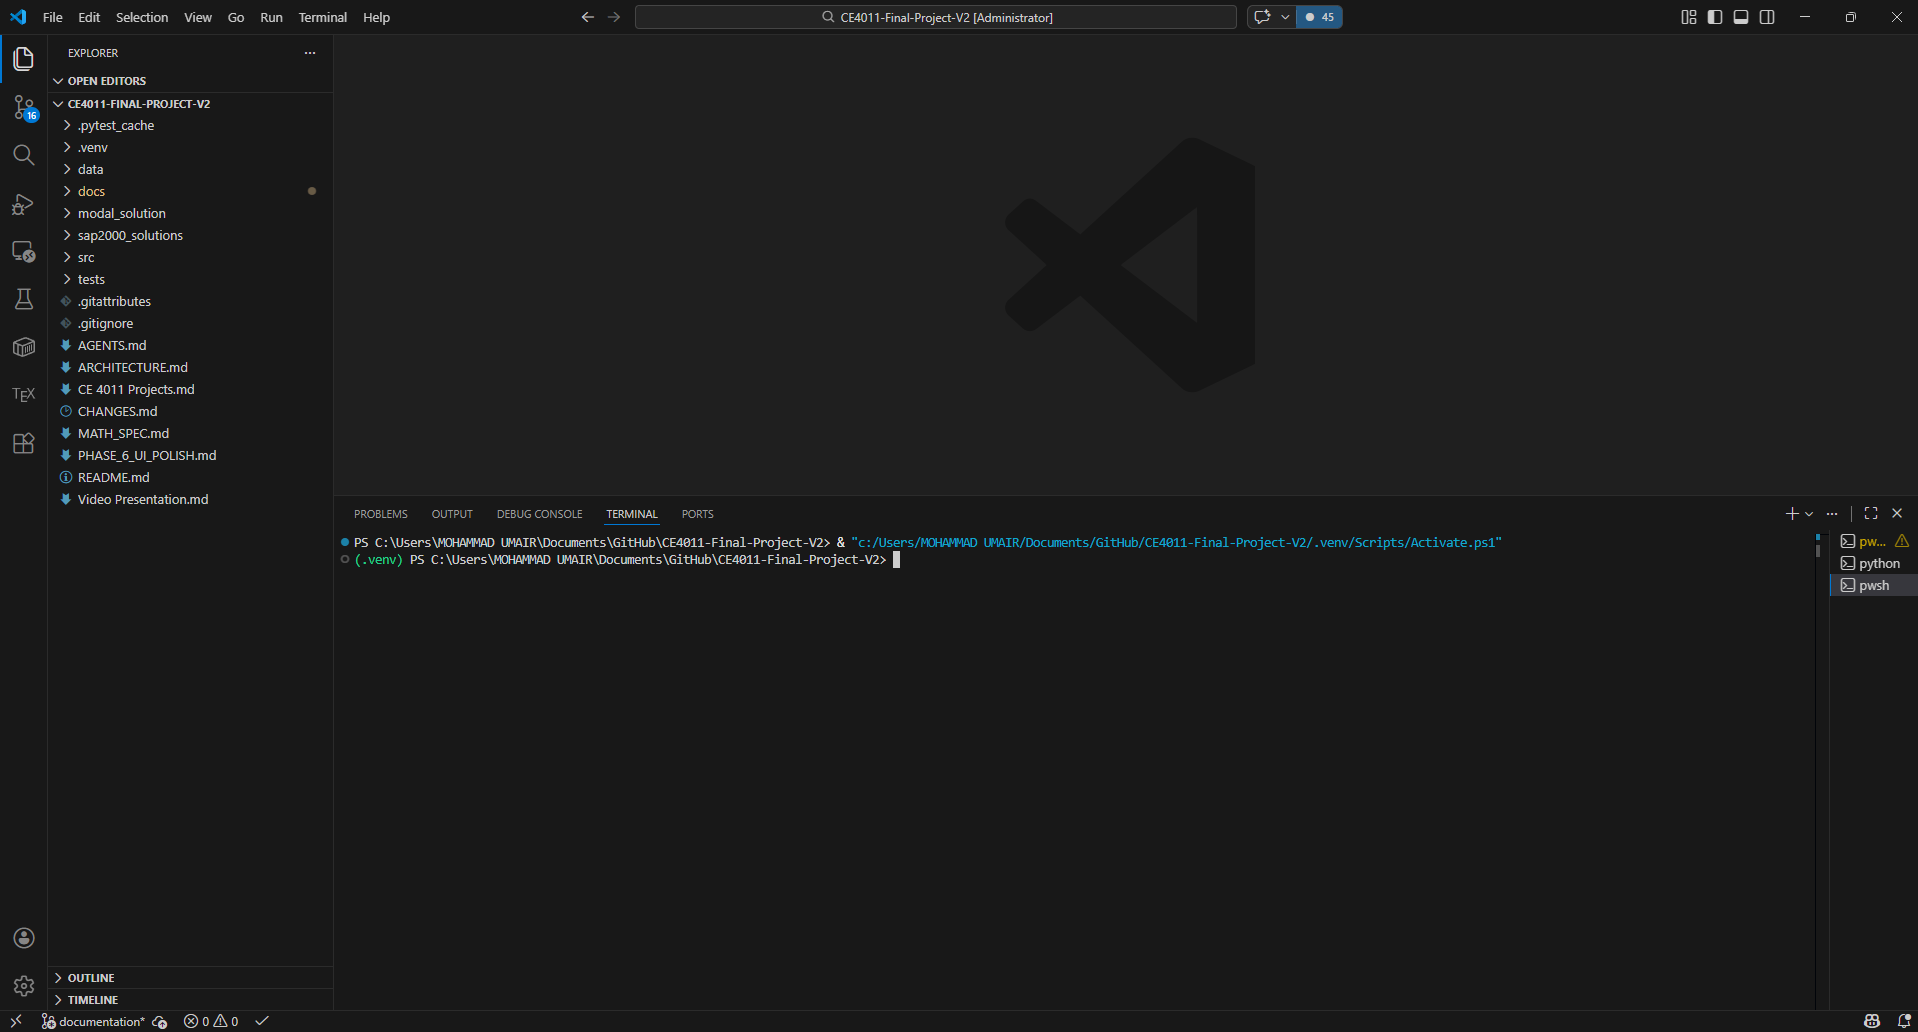
\includegraphics[width=0.92\linewidth]{figures/terminal_setup_screenshot.png}
\caption{Terminal opened at the repository root after obtaining the project folder.}
\end{figure}

\section{Virtual Environment Setup}

On Windows PowerShell:
\begin{verbatim}
python -m venv .venv
.\.venv\Scripts\Activate.ps1
python -m pip install --upgrade pip
python -m pip install matplotlib pytest
\end{verbatim}

On macOS or Linux:
\begin{verbatim}
python3 -m venv .venv
source .venv/bin/activate
python -m pip install --upgrade pip
python -m pip install matplotlib pytest
\end{verbatim}

If the command \texttt{python} points to the wrong interpreter, use the full path to the intended Python executable.

\section{Launch Command}

From the repository root, run:
\begin{verbatim}
python -m src.ui_desktop.app
\end{verbatim}

\begin{figure}[htbp]
\centering
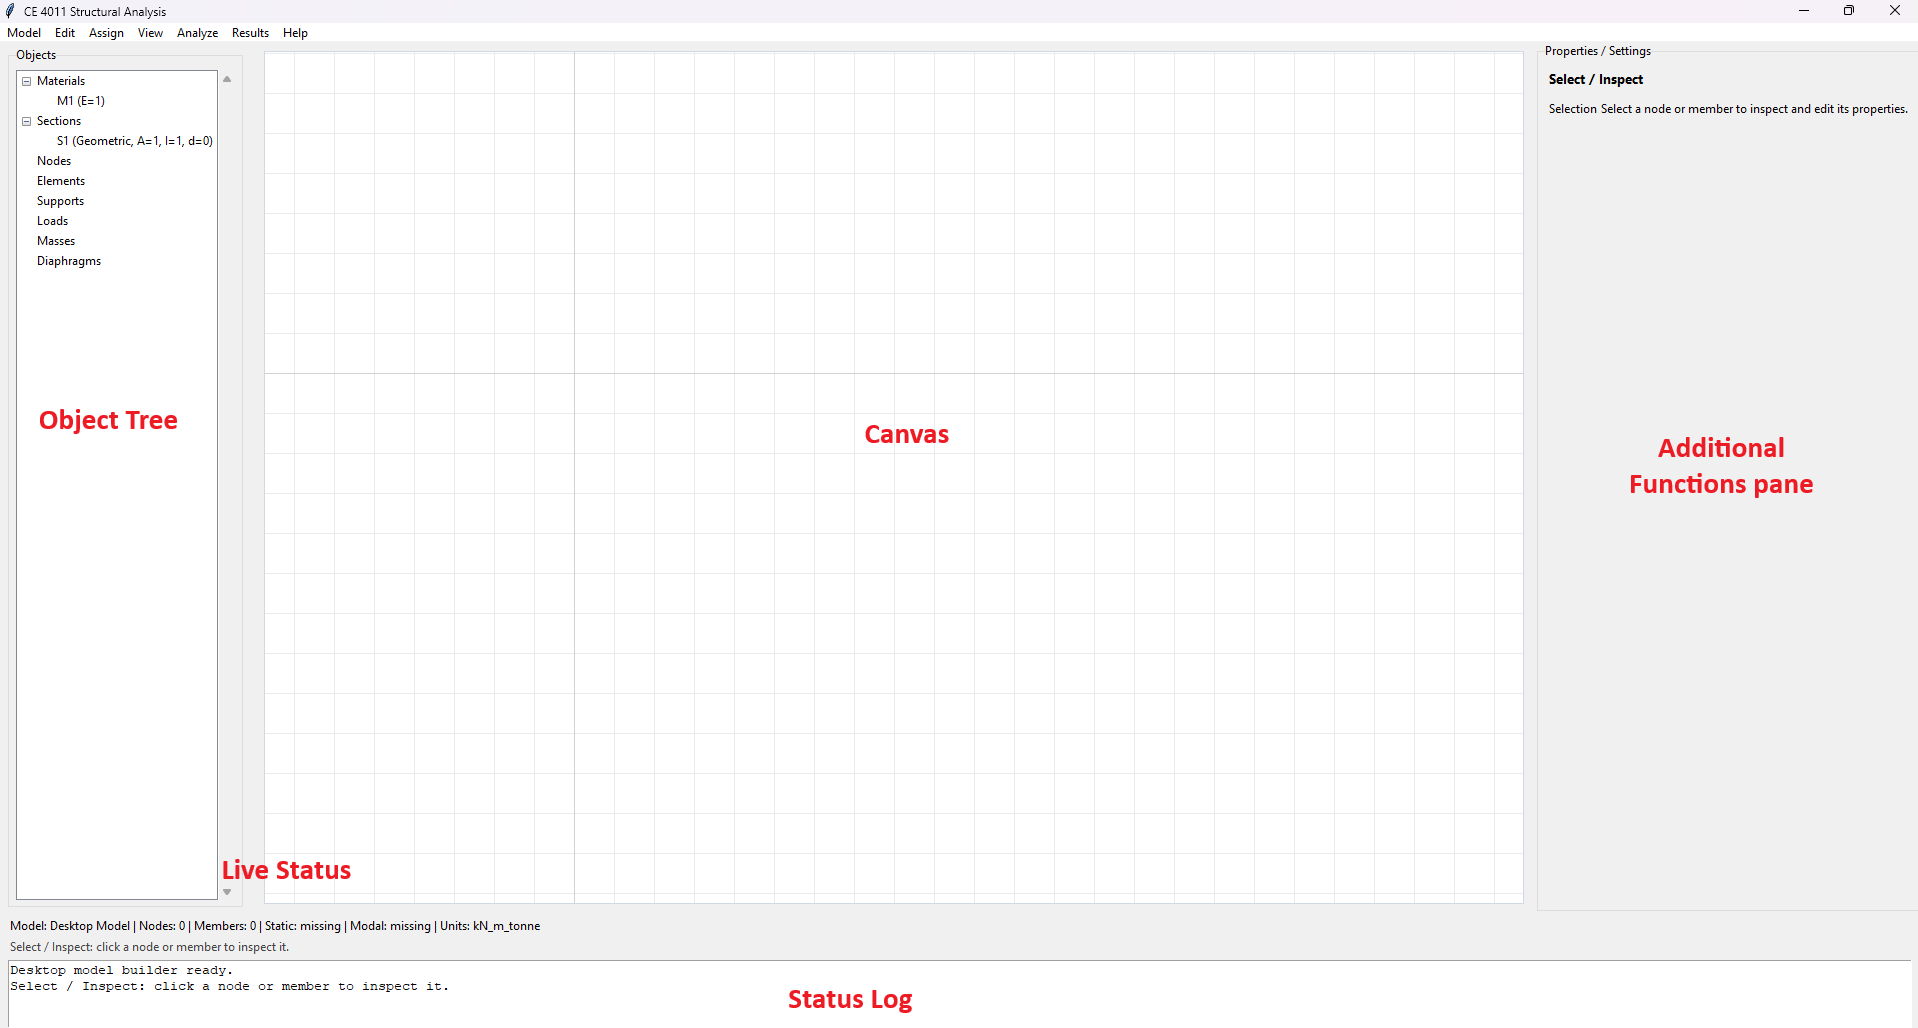
\includegraphics[width=0.92\linewidth]{figures/launched_app_screenshot.png}
\caption{Tkinter desktop application immediately after launch.}
\end{figure}

\section{Test Command}

To run the automated test suite from the repository root:
\begin{verbatim}
pytest tests/
\end{verbatim}

The final stable baseline documented for submission is \texttt{pytest tests/ -q -> 197 passed} in approximately 2 seconds.

\section{Troubleshooting}

\subsection{Wrong Working Directory}

Symptom: Python cannot find the \texttt{src} module or pytest cannot find tests.

Fix: Change directory to the repository root before running commands. The root contains \texttt{src/}, \texttt{tests/}, \texttt{data/}, and \texttt{README.md}.

\subsection{Missing Dependencies}

Symptom: Import errors for \texttt{matplotlib} or \texttt{pytest}.

Fix:
\begin{verbatim}
python -m pip install matplotlib pytest
\end{verbatim}

\subsection{Tkinter Issues}

Symptom: Import errors for \texttt{tkinter}, or the desktop window does not open.

Fix: On Windows, reinstall Python using the official installer and keep Tcl/Tk enabled. On Linux, install the distribution Tkinter package, commonly \texttt{python3-tk}, then rerun the launch command.

\subsection{matplotlib Issues}

Symptom: Plot windows or embedded plots fail to render.

Fix: Reinstall matplotlib in the active virtual environment:
\begin{verbatim}
python -m pip install --upgrade --force-reinstall matplotlib
\end{verbatim}

\subsection{pytest Not Found}

Symptom: The terminal reports that \texttt{pytest} is not recognized.

Fix: Activate the virtual environment, or run pytest through Python:
\begin{verbatim}
python -m pytest tests/
\end{verbatim}

\section{Final Scope Reminder}

Use the desktop application to create or load a model, assign supports/properties/loads/masses, validate the model, run Static or Modal analysis, inspect result tables and plots, and export visible result data where implemented. RSA and THA are future-extension work only.

\end{document}
